\documentclass[14pt,a4paper]{scrartcl}
\usepackage{cmap}
\usepackage[utf8]{inputenc}
\usepackage[T1,T2A]{fontenc}
\usepackage[english,russian]{babel}
\usepackage{relsize}
\usepackage{graphicx}
\usepackage{subfigure}
\usepackage{mathtools}
\usepackage{amssymb}
\usepackage{float}
\usepackage{sidecap}
\usepackage{wrapfig}
\usepackage{caption}
\usepackage[table,xcdraw]{xcolor}
\usepackage{minted}
\begin{document}
	\begin{titlepage}
	\begin{center}
		\large
		МИНИСТЕРСТВО НАУКИ И ВЫСШЕГО ОБРАЗОВАНИЯ\\ РОССИЙСКОЙ ФЕДЕРАЦИИ
		
		\vspace{0.5cm}
		
		МГТУ им Н.Э.Баумана
		\vspace{0.25cm}
		
		Факультет ФН
		
		Кафедра вычислительной математики и математической физики
		\vfill
		
		
		Соколов Арсений Андреевич\\
		\vfill
		
		
		{\LARGE Домашнее задание №1 \\ по теории случайных процессов\\[2mm]
		}
		\bigskip
		
		3 курс, группа ФН11-63Б\\
		Вариант 19
	\end{center}
	\vfill
	
	\newlength{\ML}
	\settowidth{\ML}{«\underline{\hspace{0.7cm}}» \underline{\hspace{2cm}}}
	\hfill\begin{minipage}{0.4\textwidth}
		Преподаватель\\
		\underline{\hspace{3cm}} Т.\,В.~Облакова\\
		«\underline{\hspace{0.7cm}}» \underline{\hspace{1.71cm}} 2019 г.
	\end{minipage}%
	\bigskip
	
	
	\vfill
	
	\begin{center}
		Москва, 2020 г.
	\end{center}
\end{titlepage}

\section*{Начальные данные}

\begin{minted}{R}
> ### Начальные данные:
> m <- 6 # Число состояний марковской цепи
> k <- 5 # время (шаги)
> n <- 180 # траектории
> set.seed(1337)
\end{minted}

\section*{Задание 1}

Смоделировать вектор начальных вероятностей $\vec{p(0)} = p(0)$ и матрицу переходных вероятностей $P$ для однородной цепи маркова с данным числом состояний ${s_1,s_2,…,s_m}$.\\
\textbf{Решение.}\\
1. Генерируем $(m+1)$ раз вектор $\vec{r}=(r_1,r_2,…,r_{m-1})$ из независимых и равномерно распределенных на отрезке $[0,1]$ случайных величин.
\begin{minted}{R}
> r_tmp <- replicate((m+1), runif((m-1), min = 0, max = 1), 
+	simplify = F)
> r_tmp
[[1]]
[1] 0.57632155 0.56474213 0.07399023 0.45386562 0.37327926

[[2]]
[1] 0.3313175 0.9476300 0.2811173 0.2454040 0.1460436

[[3]]
[1] 0.9794303 0.9937176 0.8273587 0.1939823 0.9813254

[[4]]
[1] 0.02522857 0.97238848 0.92379666 0.33913968 0.24657940

[[5]]
[1] 0.84916377 0.72408821 0.04661798 0.15367816 0.56259417

[[6]]
[1] 0.9814257 0.9317742 0.8986149 0.4697933 0.9950081

[[7]]
[1] 0.8982745 0.1016177 0.7394574 0.2291205 0.7883651
\end{minted}


2. Для каждого из полученных векторов строим вариационный ряд, то есть упорядочиваем по возрастанию.

\begin{minted}{R}
> r <- lapply(r_tmp, sort)
> r
[[1]]
[1] 0.07399023 0.37327926 0.45386562 0.56474213 0.57632155

[[2]]
[1] 0.1460436 0.2454040 0.2811173 0.3313175 0.9476300

[[3]]
[1] 0.1939823 0.8273587 0.9794303 0.9813254 0.9937176

[[4]]
[1] 0.02522857 0.24657940 0.33913968 0.92379666 0.97238848

[[5]]
[1] 0.04661798 0.15367816 0.56259417 0.72408821 0.84916377

[[6]]
[1] 0.4697933 0.8986149 0.9317742 0.9814257 0.9950081

[[7]]
[1] 0.1016177 0.2291205 0.7394574 0.7883651 0.8982745
\end{minted}

3. Находим длины отрезков, на которые вектор $\vec{r}$ разбивает отрезок $[0;1]$ -- получаем вектор вероятностей $\vec{p}$.

\begin{minted}{R}
> p_tmp <- lapply(r, diff)
> 
> heads <- lapply(r, head, 1)
> tails <- lapply(r, function(x) (1-tail(x,1)))
> 
> p <- mapply(append, mapply(append, heads,p_tmp,SIMPLIFY = F),
+             tails, SIMPLIFY = F)
> p
[[1]]
[1] 0.07399023 0.29928903 0.08058636 0.11087650 0.01157942 0.42367845

[[2]]
[1] 0.14604362 0.09936043 0.03571326 0.05020014 0.61631257 0.05236998

[[3]]
[1] 0.193982297 0.633376436 0.152071561 0.001895136 0.012392162 0.00628241

[[4]]
[1] 0.02522857 0.22135084 0.09256028 0.58465698 0.04859183 0.02761152

[[5]]
[1] 0.04661798 0.10706018 0.40891601 0.16149404 0.12507555 0.15083623

[[6]]
[1] 0.469793260 0.428821684 0.033159286 0.049651461 0.013582420 0.00499190

[[7]]
[1] 0.10161771 0.12750281 0.51033685 0.04890769 0.10990946 0.10172548
\end{minted}

Проверим, что полученные вектора обладают свойством стохастичности:

\begin{minted}{R}
> mapply(sum, p)
[1] 1 1 1 1 1 1 1
\end{minted}

Получили, что сумма элементов каждого вектора $\vec{p}$ равна единице.

4. Первый из полученных векторов $\vec{p}$ считаем вектором начальных вероятностей, из остальных составляем матрицу переходов $P$, записывая их по строкам.

\begin{minted}{R}
> p0 <- p[[1]] # вектор начальных условий
> p0
[1] 0.07399023 0.29928903 0.08058636 0.11087650 0.01157942 0.42367845
> P <- t(simplify2array(p))[-1,] # матрица переходов
> P
           [,1]       [,2]       [,3]        [,4]       [,5]        [,6]
[1,] 0.14604362 0.09936043 0.03571326 0.050200143 0.61631257 0.052369977
[2,] 0.19398230 0.63337644 0.15207156 0.001895136 0.01239216 0.006282408
[3,] 0.02522857 0.22135084 0.09256028 0.584656978 0.04859183 0.027611518
[4,] 0.04661798 0.10706018 0.40891601 0.161494042 0.12507555 0.150836234
[5,] 0.46979326 0.42882168 0.03315929 0.049651461 0.01358242 0.004991889
[6,] 0.10161771 0.12750281 0.51033685 0.048907685 0.10990946 0.101725481
\end{minted}

\pagebreak
\section*{Задание 2}
Построить размеченный граф состояний цепи.\\
\textbf{Решение.}\\

\begin{minted}{R}
> library(markovchain)
> library(diagram)
> 
> png(filename = "../img/1.png",
+     width = 1920, height = 1080,
+     res = 96 * 1.25)
> plotmat(signif(P,3), 
+         lwd = 1, box.lwd = 2, 
+         cex.txt = 0.8, 
+         box.size = 0.04, 
+         box.type = "circle", 
+         box.prop = 0.5,
+         box.col = "light blue",
+         arr.length=.25,
+         arr.width=.1,
+         self.cex = .7,
+         self.shifty = -.01,
+         self.shiftx = .07,
+         main = "Markov Chain")
> dev.off()
\end{minted}

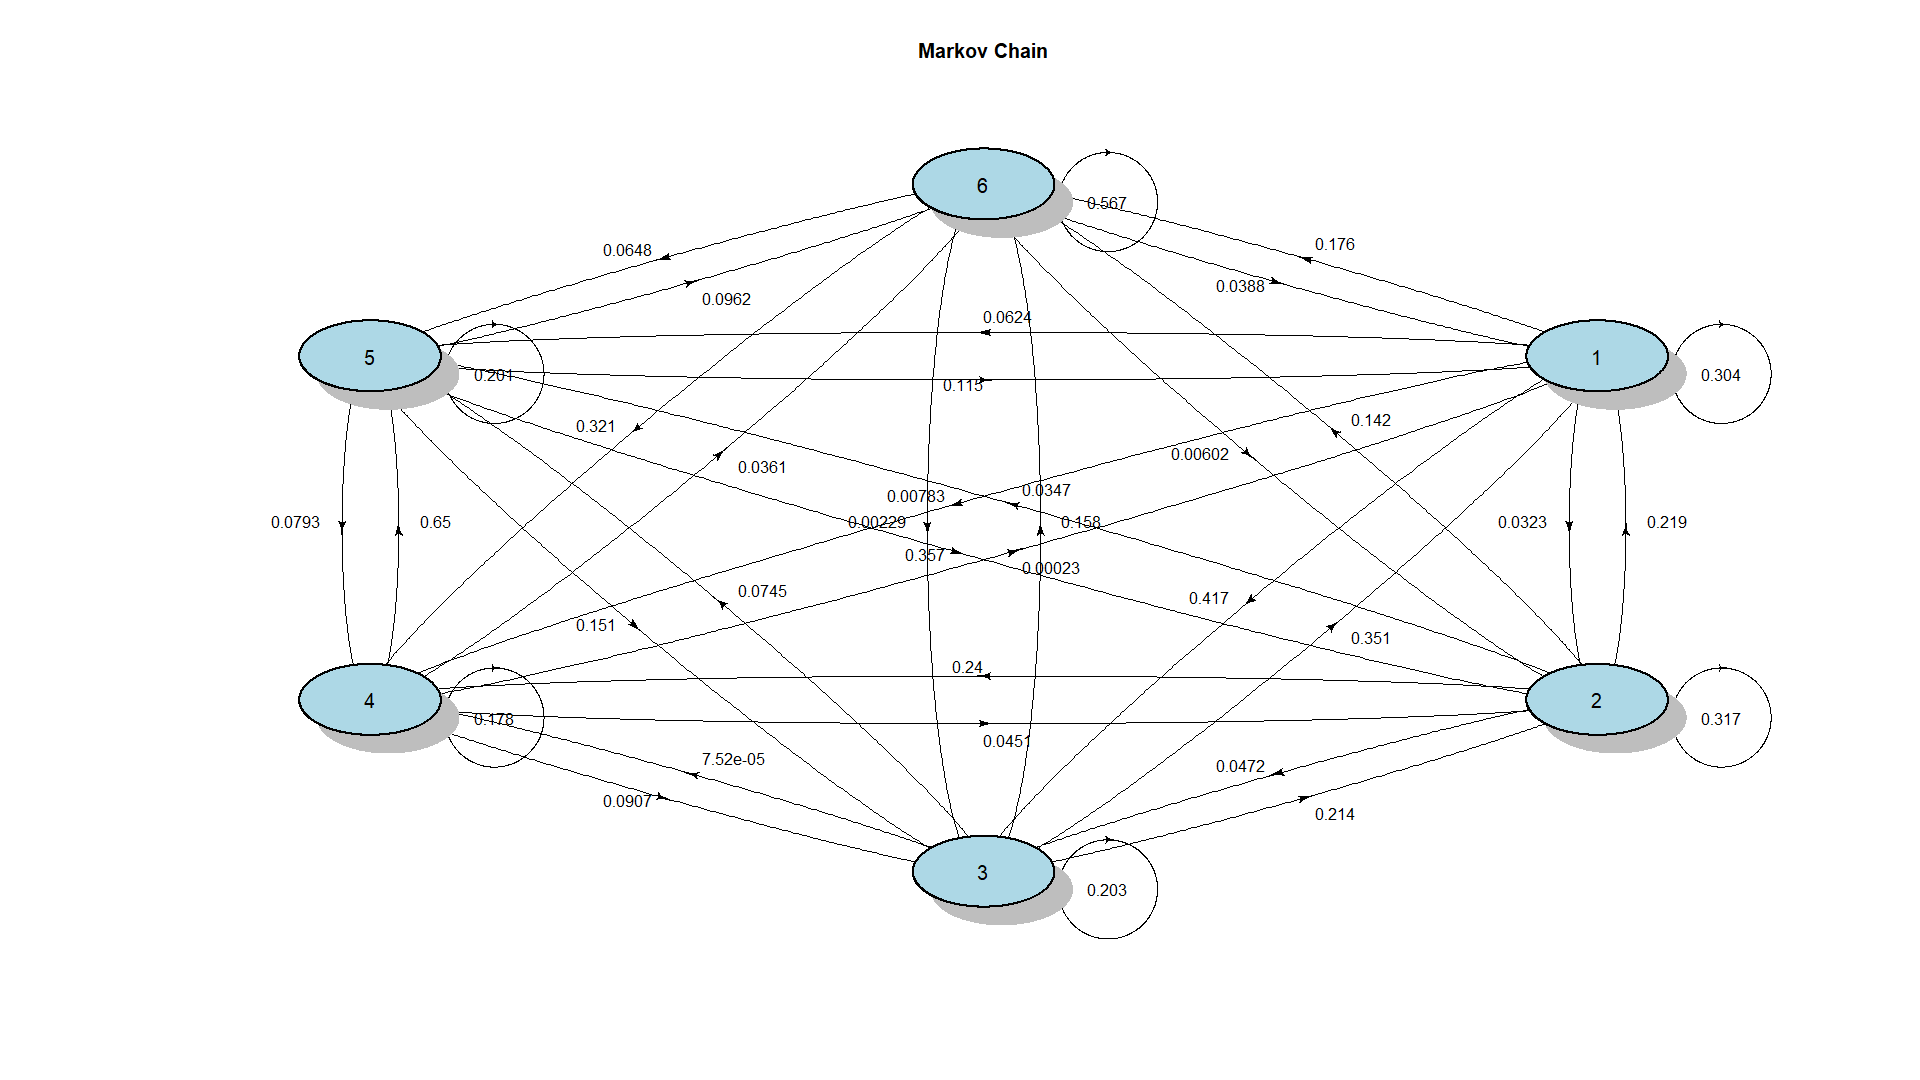
\includegraphics[angle=90,origin=t, scale=0.75]{../img/1.png}

\pagebreak

\section*{Задание 3.}
Вычислить безусловные вероятности состояний смоделированной цепи на k шаге.\\
\textbf{Решение.}\\

\begin{minted}{R}
> library(matrixcalc)
> p_k <- p0 %*% matrix.power(P,k)
> p_k
	[,1]      [,2]      [,3]      [,4]     [,5]      [,6]
[1,] 0.170569 0.3514299 0.1596612 0.1356754 0.1402044 0.04246026
\end{minted}

А также для некоторых других значений $k$:
\begin{minted}{R}
> p_k2 <- p0 %*% matrix.power(P,2)
> p_k2
	[,1]      [,2]      [,3]      [,4]      [,5]       [,6]
[1,] 0.1461953 0.3307245 0.1527279 0.2160571 0.1160726 0.03822257

> p_k3 <- p0 %*% matrix.power(P,3)
> p_k3
	[,1]      [,2]      [,3]      [,4]      [,5]       [,6]
[1,] 0.1578451 0.3355846 0.1813559 0.1397837 0.1344228 0.05100792

> p_k4 <- p0 %*% matrix.power(P,4)
> p_k4
	[,1]      [,2]      [,3]     [,4]      [,5]       [,6]
[1,] 0.1675757 0.3474905 0.1611048 0.146334 0.1351685 0.04232641

> p_k5 <- p0 %*% matrix.power(P,5)
> p_k5
	[,1]      [,2]      [,3]      [,4]      [,5]       [,6]
[1,] 0.170569 0.3514299 0.1596612 0.1356754 0.1402044 0.04246026

> p_k10 <- p0 %*% matrix.power(P,10)
> p_k10
	[,1]      [,2]      [,3]      [,4]      [,5]       [,6]
[1,] 0.1762364 0.3585034 0.1531416 0.1291872 0.1428944 0.04003696

> p_k100 <- p0 %*% matrix.power(P,100)
> p_k100
	[,1]      [,2]      [,3]      [,4]      [,5]       [,6]
[1,] 0.1765572 0.3589433 0.1527727 0.1287059 0.1431139 0.03990709
\end{minted}

\section*{Задание 4}
Смоделировать $n$ траекторий полученной цепи за $k$ шагов и найти вектор относительных частот ее состояний на $k$ шаге.\\
\textbf{Решение.}\\

1. Генерируем равномерно распределенную на $[0;1]$ случайную величину $r_0$ и по вектору $\vec{r_1}$ разыгрываем начальное состояние следующим образом: если $r_0 < r_{1_1}$, то полагаем, что $\xi_0 = s_1 = 1$, если $r_0 < r_{1_2}$, то полагаем, что $\xi_0 = s_2 = 2$, \ldots, если $r_0 < r_{1_{m-1}}$, то полагаем, что $\xi_0 = s_{m-1} = m-1$, иначе если $r_0 > r_{1_{m-1}}$, то полагаем, что $\xi_0 = s_{m} = m = j_0$.


\begin{minted}{R}
> r0 <- runif(1, min = 0, max = 1)
> r0
[1] 0.4436541
> foo <- function(r0_loc,j)
+   {
+     ifelse(r0_loc < r[[j+1]][1],1,
+     ifelse(r0_loc < r[[j+1]][2],2,
+     ifelse(r0_loc < r[[j+1]][3],3,
+     ifelse(r0_loc < r[[j+1]][4],4,
+     ifelse(r0_loc < r[[j+1]][5],5,6)))))
+   }
>   
>   step_1 <- foo(r0,1)
> step_1
[1] 3
###
> r[[1]]
[1] 0.07399023 0.37327926 0.45386562 0.56474213 0.57632155
\end{minted}

Разыгранное число $r_0 = 0.4436541$, что меньше, чем 4-эй элемент $r_1$, но больше, чем 2-эй, то есть $(0.37327926 = r_{1_2}) < 0.4436541 < (0.56474213 = r_{1_4})  \Rightarrow \xi_0 = 3$. \\

2. Генерируем ещё одно значение $r_1$ и по строке с номером $j_0 = 3$ аналогично предыдущему пункту разыгрываем значение $\xi_1:$

\begin{minted}{R}
> r1 <- runif(1, min = 0, max = 1)
> r1
[1] 0.930468
> step_2 <- foo(r1,step_1)
> step_2
[1] 5
\end{minted}

3. Повторяем алгоритм  заданное число раз $k$.

\begin{minted}{R}
> r2 <- runif(1, min = 0, max = 1)
> r2
[1] 0.6091826
> step_3 <- foo(r2,step_2)
> step_3
[1] 2
> r3 <- runif(1, min = 0, max = 1)
> r3
[1] 0.4071127
> step_4 <- foo(r3,step_3)
> step_4
[1] 2
> r4 <- runif(1, min = 0, max = 1)
> r4
[1] 0.8295361
> step_5 <- foo(r4,step_4)
> step_5
[1] 3
> r5 <- runif(1, min = 0, max = 1)
> r5
[1] 0.9402458
> step_6 <- foo(r5,step_5)
> step_6
[1] 5
\end{minted}

Получаем выборочную траекторию цепи:

\begin{minted}{R}
> c(step_1,step_2,step_3,step_4,step_5,step6)
[1] 3 5 2 2 3 5
\end{minted}
	
4. Повторяем процедуру 1-3 $n$ число раз.

Полученный выше вектор подробно описан для одной итерации. В общем виде алгоритм выглядит, как представлено ниже в листинге. Очевидно, что вектор из предыдущего пункта не является первым вектором в получаемом ниже списке траекторий, так как использован только в качестве примера. В общем виде цикл итерируется от 1 до $n$ и первая траектория не будет равна той, что получена выше, так как будет перезаписана первой итерацией цикла.
\pagebreak
\begin{minted}{R}
tracs <- list()
for (i in 1:n)
{
	r0 <- runif(1, min = 0, max = 1)
	foo <- function(r0_loc,j)
	{
		ifelse(r0_loc < r[[j+1]][1],1,
		ifelse(r0_loc < r[[j+1]][2],2,
		ifelse(r0_loc < r[[j+1]][3],3,
		ifelse(r0_loc < r[[j+1]][4],4,
		ifelse(r0_loc < r[[j+1]][5],5,6)))))
	}
	step_1 <- foo(r0,0)
	step_2 <- foo(runif(1, min = 0, max = 1),step_1)
	step_3 <- foo(runif(1, min = 0, max = 1),step_2)
	step_4 <- foo(runif(1, min = 0, max = 1),step_3)
	step_5 <- foo(runif(1, min = 0, max = 1),step_4)
	trac <- list(c(step_1,step_2,step_3,step_4,step_5,step_6))
	tracs[k] <- trac
}

tracs_array <- t(simplify2array(tracs,higher = F))
colnames(tracs_array) <- paste("Шаг",as.character(0:k))
rownames(tracs_array) <- paste("Тр.",as.character(1:n))
\end{minted}

В итоге получаем $n=180$ штук траекторий длины $k=5$.

Посмотрим на первые и последние 5 траекторий:

\begin{minted}{R}
> head(tracs_array,5)
	Шаг 0 Шаг 1 Шаг 2 Шаг 3 Шаг 4 Шаг 5
Тр. 1     2     3     3     5     2     2
Тр. 2     6     3     4     4     4     1
Тр. 3     3     6     3     4     5     2
Тр. 4     3     4     2     3     4     5
Тр. 5     2     1     5     2     2     1
> tail(tracs_array,5)
	Шаг 0 Шаг 1 Шаг 2 Шаг 3 Шаг 4 Шаг 5
Тр. 176     3     2     1     1     5     1
Тр. 177     2     3     4     2     1     1
Тр. 178     2     1     5     2     3     4
Тр. 179     2     1     1     2     2     2
Тр. 180     3     4     6     5     1     5
\end{minted}



\section*{Задание 5}
Вычислить эмпирические вероятности (относительные частоты) состояний  цепи на $k$ шаге.\\
\textbf{Решение.}\\

Рассмотрим $k-$ый шаг ($k=5$). Посчитаем количество $n_j$ смоделированных траекторий, находящихся в состоянии $s_j$ на $k-$ом шаге. Поделив на общее число $n=180$ траекторий, получим эмпирические вероятности. 

\begin{minted}{R}
> hist(tracs_array[,k+1], breaks =0:m)$counts
[1] 32 67 30 21 21  9
> emp <- hist(tracs_array[,k], breaks =0:m)$density
> emp
[1] 0.16666667 0.41111111 0.11666667 0.15555556 0.12222222 0.02777778
\end{minted}

Сравним полученные эмпирические вероятности с вектором $\vec{p_k}$, полученным в 3 пункте. Для этого построим группированные bar-plots:

\begin{minted}{R}
> plot_df <- data.frame(type = rep(c("theoretical", "emperical"), each=m),
+                       state = rep(paste("S",as.character(1:m),
+										  sep = "_"), 2),
+                       prob = c(theor, emp))
> 
> png(filename = "../img/2.png",
+     width = 1920, height = 1080,
+     res = 96 * 2)
> ggplot(data=plot_df, aes(x=state, y=prob, fill=type)) +
+   geom_bar(stat="identity", position=position_dodge()) + 
+   theme_bw() + ggtitle("Шаг 5")
> dev.off()
\end{minted}

\begin{figure}[H]
	\begin{minipage}[h]{1\linewidth}
		\center{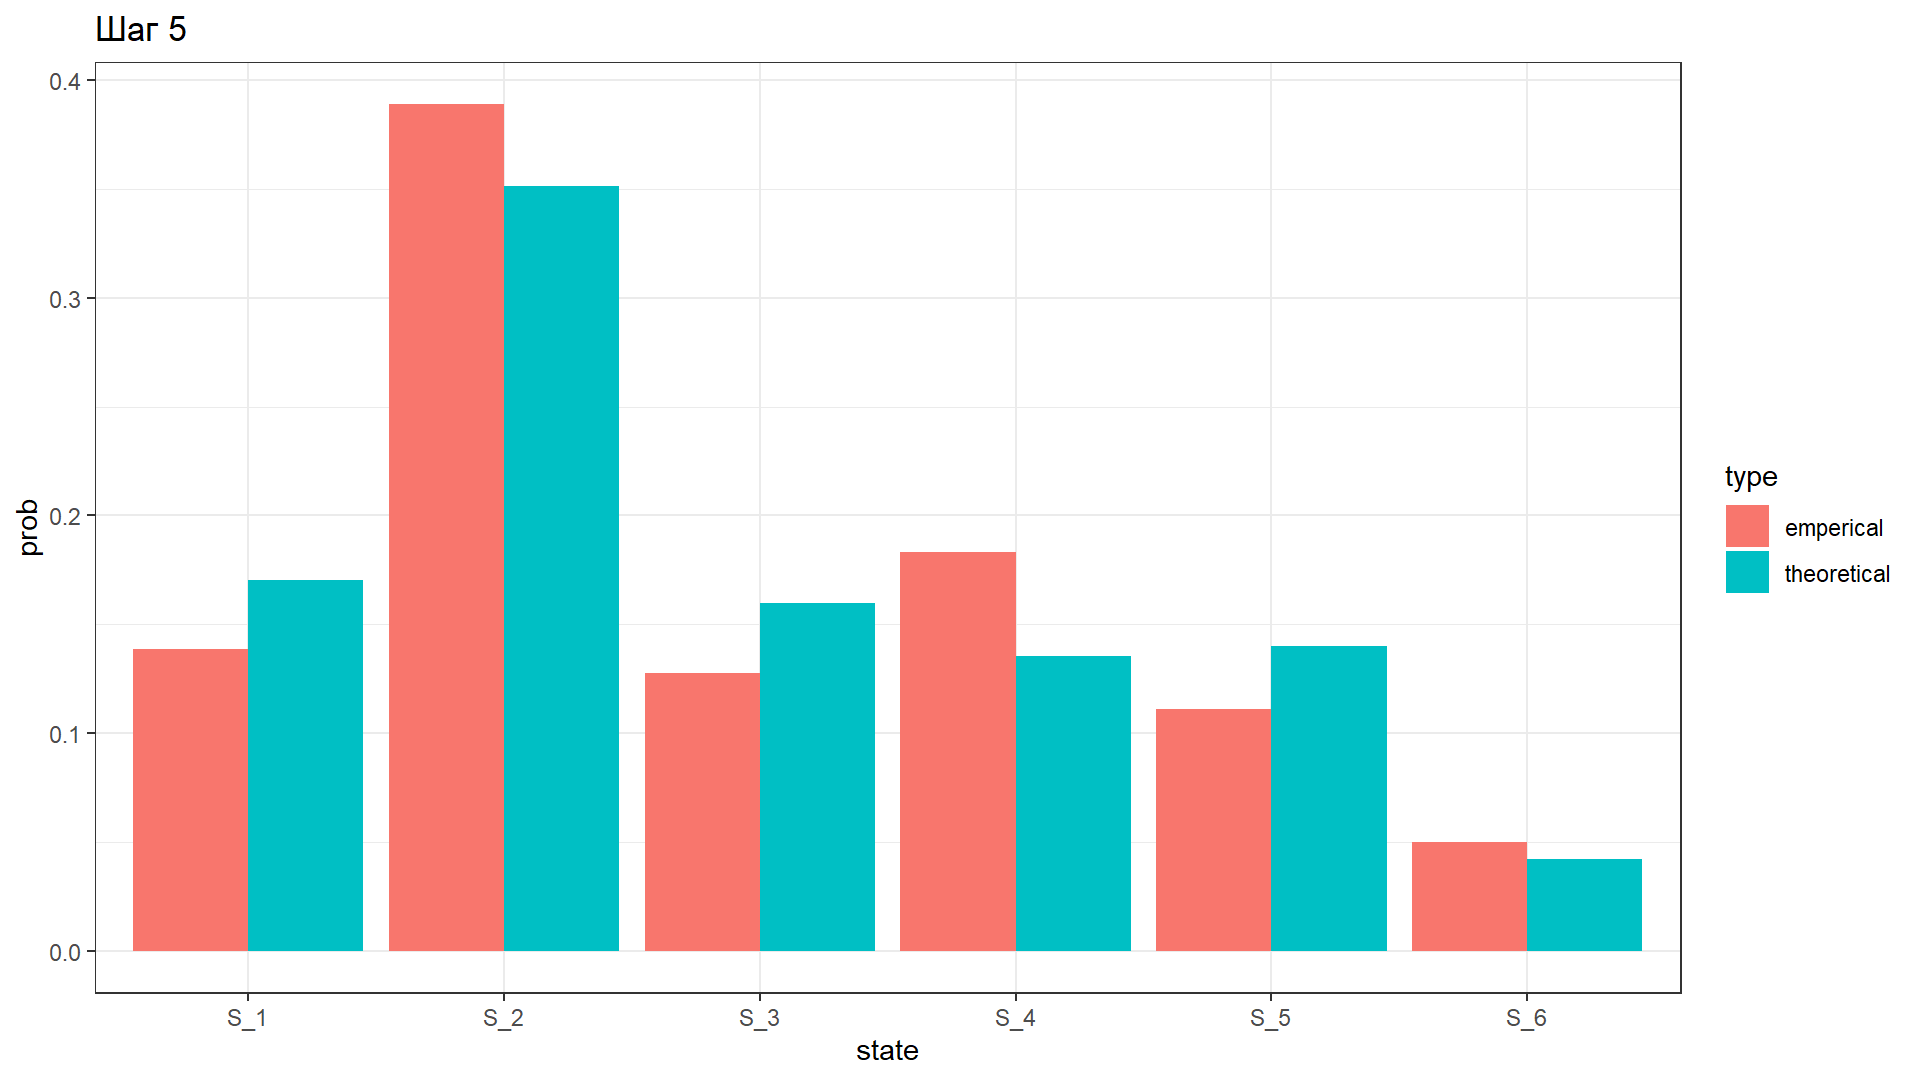
\includegraphics[width=1\linewidth]{../img/2.png}}  \\
	\end{minipage}
\end{figure}


Рассмотрим разности соответствующих значений эмпирической и теоретической вероятностей, а также максимальное по модулю значение разности:

\begin{minted}{R}
> emp
[1] 0.16666667 0.41111111 0.11666667 0.15555556 0.12222222 0.02777778
> theor
[1] 0.17056898 0.35142986 0.15966116 0.13567537 0.14020437 0.04246026
> prob_diff <- emp - theor
> signif(prob_diff,5)
[1] -0.0039023  0.0596810 -0.0429940  0.0198800 -0.0179820 -0.0146820
 # Округлено до 5 значащих знаков, чтобы влезало в страницу
> max(abs(prob_diff))
[1] 0.05968125
\end{minted}

Дополнительно построим для первых 5-и траекторий группированный bar-plot. По оси абсцисс представлены шаги (от $0$ до $k$), по оси ординат -- состояния (от $1$ до $m$).

\begin{minted}{R}
> plot_df_obl <- data.frame(
+               type = rep(c("Тр. 1", "Тр. 2", "Тр. 3", "Тр. 4"), each=m),
+               step = rep(paste("Шаг",as.character(0:k),sep = " "), 2),
+               state = c(tracs_array[1,], tracs_array[2,], 
+                                tracs_array[3,], tracs_array[4,]))
> png(filename = "../img/3.png",
+     width = 1920, height = 1080,
+     res = 96 * 2)
> ggplot(data=plot_df_obl, aes(x=step, y=state, fill=type)) +
+   geom_bar(stat="identity", position=position_dodge()) +
+   scale_fill_manual("legend", 
+   values = 
+	c("#03A82F", "#07728C", "#E17204", "#E11E04", "#EAD497")) +
+   theme_bw()
> dev.off()
\end{minted}

\begin{figure}[H]
	\begin{minipage}[h]{1\linewidth}
		\center{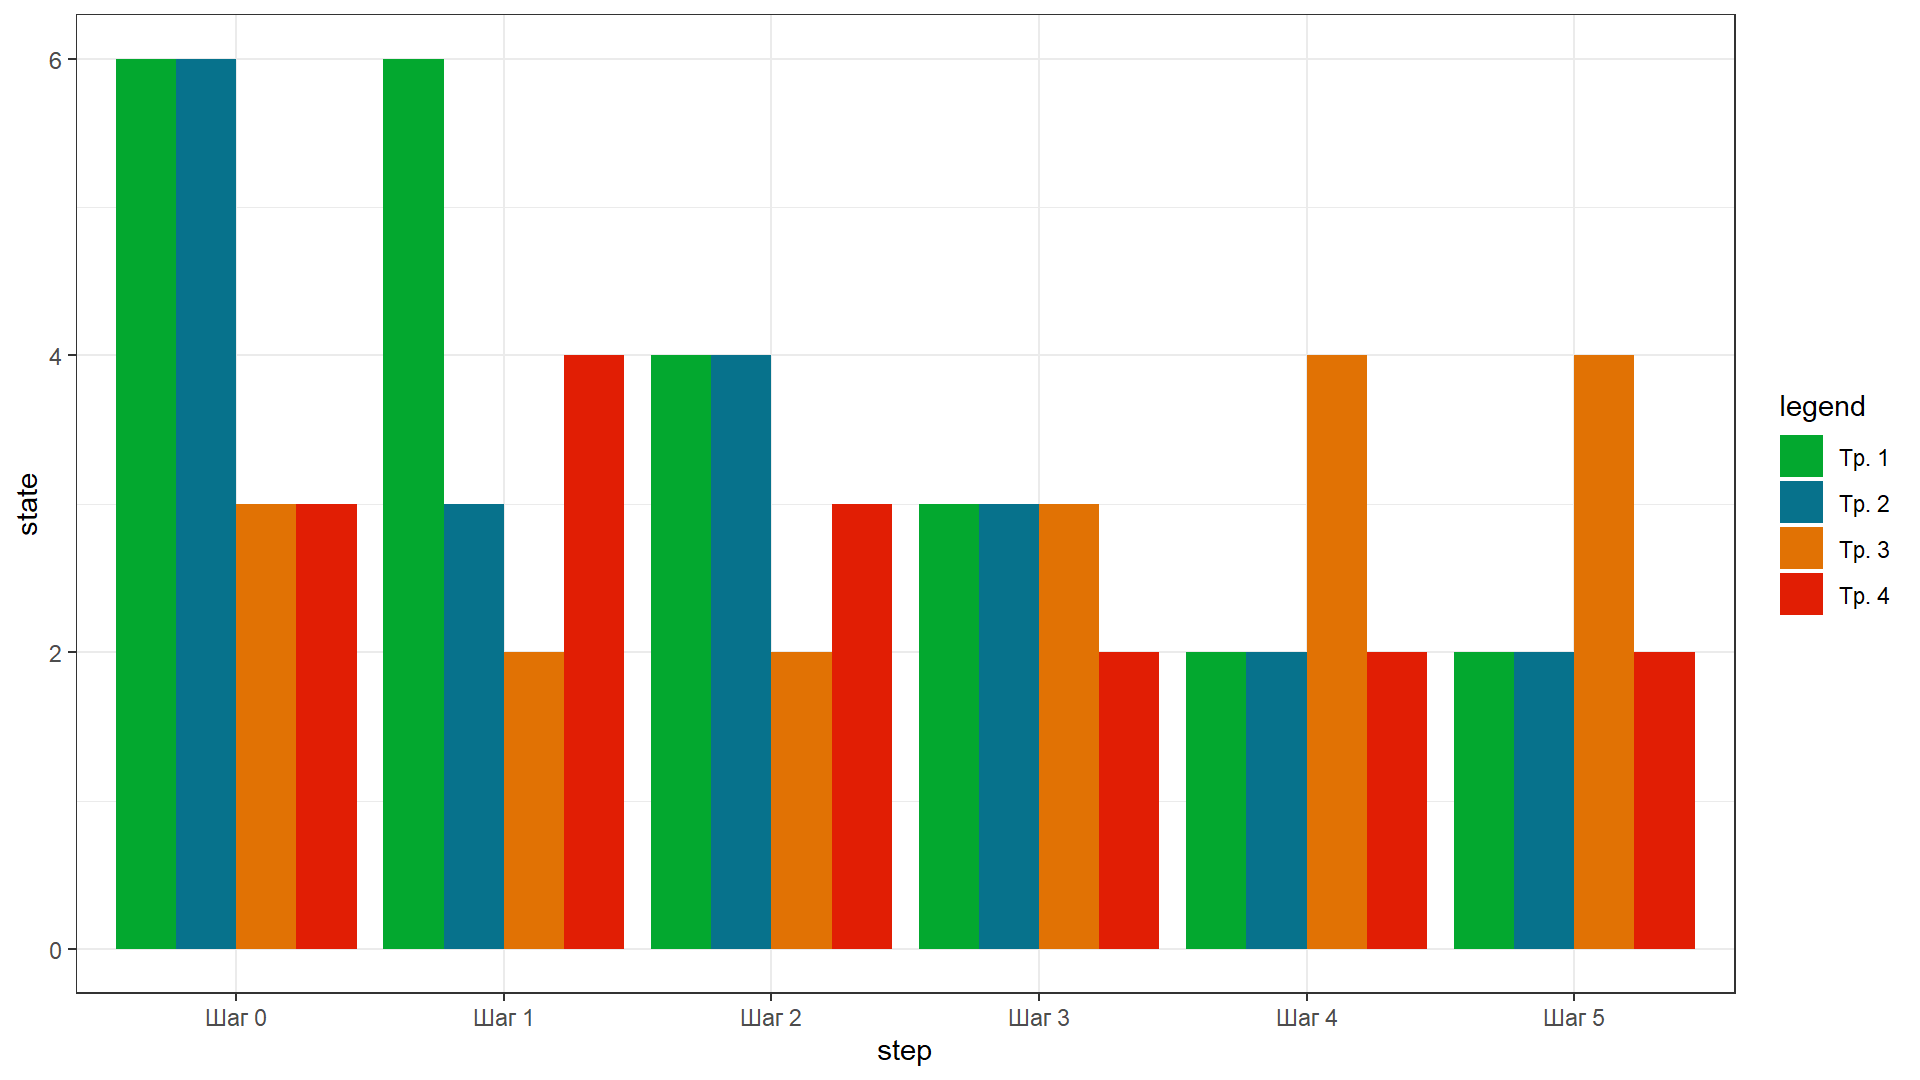
\includegraphics[width=1.1\linewidth]{../img/3.png}}  \\
	\end{minipage}
\end{figure}

\begin{minted}{R}
> head(tracs_array,4)
	Шаг 0 Шаг 1 Шаг 2 Шаг 3 Шаг 4 Шаг 5
Тр. 1     6     6     4     3     2     2
Тр. 2     6     3     4     3     2     2
Тр. 3     3     2     2     3     4     4
Тр. 4     3     4     3     2     2     2
\end{minted}

\pagebreak
\section*{Задание 6}
Вычислить финальные вероятности для марковской цепи и сравнить их  вероятностями состояний на $k$ шаге.\\
\textbf{Решение.}\\

Для нахождения финальных вероятностей марковской цепи рассмотрим систему:
\begin{equation*}
	\begin{cases} 
		\sum\limits_{i=1}^m \pi_i P_{i,j} = \pi_j\\ 
		\sum\limits_{i=1}^m \pi_i = 1\\ 
	\end{cases}
\end{equation*}

Вычёркивая последнюю строчку транспонированной $P$, из которой вычтена единичная матрица, и дописывая балансное уравнение, получаем систему (округлено до 3 значащих знаков):
\begin{equation*}
	\resizebox{0.91\hsize}{!}
	{
		$\begin{array}{lllllllllllll}
		-0.854 \cdot \pi1  &+& 0.194 \cdot \pi2 &+& 0.0252 \cdot \pi3 &+& 0.0466 \cdot \pi4   &+& 0.47 \cdot \pi5  &+& 0.102 \cdot \pi6  &=&  0 \\ 
		0.0994 \cdot \pi1  &-& 0.367 \cdot \pi2  &+& 0.221 \cdot \pi3  &+& 0.107 \cdot \pi4  &+& 0.429 \cdot \pi5  &+& 0.128 \cdot \pi6  &=&  0 \\ 
		0.0357 \cdot \pi1  &+& 0.152 \cdot \pi2  &-& 0.907 \cdot \pi3  &+& 0.409 \cdot \pi4 &+& 0.0332 \cdot \pi5   &+& 0.51 \cdot \pi6  &=&  0 \\ 
		0.0502 \cdot \pi1 &+& 0.0019 \cdot \pi2  &+& 0.585 \cdot \pi3  &-& 0.839 \cdot \pi4 &+& 0.0497 \cdot \pi5 &+& 0.0489 \cdot \pi6  &=&  0 \\ 
		0.616 \cdot \pi1 &+& 0.0124 \cdot \pi2 &+& 0.0486 \cdot \pi3  &+& 0.125 \cdot \pi4  &-& 0.986 \cdot \pi5   &+& 0.11 \cdot \pi6  &=&  0 \\ 
		1 \cdot \pi1      &+& 1 \cdot \pi2      &+& 1 \cdot \pi3      &+& 1 \cdot \pi4      &+& 1 \cdot \pi5      &+& 1 \cdot \pi6  &=&  1 \\ 
		\end{array}$
	}
\end{equation*}

Решаем полученную систему:


\begin{minted}{R}
> b <- c(rep(0,m-1),1)
> b
[1] 0 0 0 0 0 1
> maat <- rbind((t(P) - diag(m))[-m,],rep(1,m))
> round(maat,7) # Округлено до 7 знаков после запятой
	[,1]       [,2]       [,3]       [,4]       [,5]      [,6]
[1,] -0.8539564  0.1939823  0.0252286  0.0466180  0.4697933 0.1016177
[2,]  0.0993604 -0.3666236  0.2213508  0.1070602  0.4288217 0.1275028
[3,]  0.0357133  0.1520716 -0.9074397  0.4089160  0.0331593 0.5103369
[4,]  0.0502001  0.0018951  0.5846570 -0.8385060  0.0496515 0.0489077
[5,]  0.6163126  0.0123922  0.0485918  0.1250756 -0.9864176 0.1099095
[6,]  1.0000000  1.0000000  1.0000000  1.0000000  1.0000000 1.0000000
> res <- solve(maat,b)
> res
[1] 0.17655716 0.35894326 0.15277268 0.12870587 0.14311394 0.03990709
\end{minted}

\pagebreak
Сравниваем со значением $\vec{p_k}$:
\begin{minted}{R}
> res
[1] 0.17655716 0.35894326 0.15277268 0.12870587 0.14311394 0.03990709
> as.numeric(p_k)
[1] 0.17056898 0.35142986 0.15966116 0.13567537 0.14020437 0.04246026
> res - as.numeric(p_k)
[1]  0.005988178  0.007513395 -0.006888475
[4] -0.006969505  0.002909572 -0.002553164
> max(abs(res-as.numeric(p_k)))
[1] 0.007513395
\end{minted}















\end{document}